\documentclass{article}

% if you need to pass options to natbib, use, e.g.:
%     \PassOptionsToPackage{numbers, compress}{natbib}
% before loading neurips_2026

% The authors should use one of these tracks.
% Before accepting by the NeurIPS conference, select one of the options below.
% 0. "default" for submission
\usepackage[final]{neurips_2026}
% the "default" option is equal to the "main" option, which is used for the Main Track with double-blind reviewing.
% 1. "main" option is used for the Main Track
%  \usepackage[main]{neurips_2026}
% 2. "position" option is used for the Position Paper Track
%  \usepackage[position]{neurips_2026}
% 3. "eandd" option is used for the Evaluations & Datasets Track
 % \usepackage[eandd]{neurips_2026}
 % if you need to opt-in for a single-blind submission in the E&D track:
 %\usepackage[eandd, nonanonymous]{neurips_2026}
% 4. "creativeai" option is used for the Creative AI Track
%  \usepackage[creativeai]{neurips_2026}
% 5. "sglblindworkshop" option is used for the Workshop with single-blind reviewing
 % \usepackage[sglblindworkshop]{neurips_2026}
% 6. "dblblindworkshop" option is used for the Workshop with double-blind reviewing
%  \usepackage[dblblindworkshop]{neurips_2026}

% After being accepted, the authors should add "final" behind the track to compile a camera-ready version.
% 1. Main Track
 % \usepackage[main, final]{neurips_2026}
% 2. Position Paper Track
%  \usepackage[position, final]{neurips_2026}
% 3. Evaluations & Datasets Track
 % \usepackage[eandd, final]{neurips_2026}
% 4. Creative AI Track
%  \usepackage[creativeai, final]{neurips_2026}
% 5. Workshop with single-blind reviewing
%  \usepackage[sglblindworkshop, final]{neurips_2026}
% 6. Workshop with double-blind reviewing
%  \usepackage[dblblindworkshop, final]{neurips_2026}
% Note. For the workshop paper template, both \title{} and \workshoptitle{} are required, with the former indicating the paper title shown in the title and the latter indicating the workshop title displayed in the footnote.
% For workshops (5., 6.), the authors should add the name of the workshop, "\workshoptitle" command is used to set the workshop title.
% \workshoptitle{WORKSHOP TITLE}

% "preprint" option is used for arXiv or other preprint submissions
 % \usepackage[preprint]{neurips_2026}

% to avoid loading the natbib package, add option nonatbib:
%    \usepackage[nonatbib]{neurips_2026}

\usepackage[utf8]{inputenc} % allow utf-8 input
\usepackage[T1]{fontenc}    % use 8-bit T1 fonts
\usepackage{hyperref}       % hyperlinks
\usepackage{url}            % simple URL typesetting
\usepackage{booktabs}       % professional-quality tables
\usepackage{amsfonts}       % blackboard math symbols
\usepackage{nicefrac}       % compact symbols for 1/2, etc.
\usepackage{microtype}      % microtypography
\usepackage{xcolor}         % colors
\usepackage{graphicx}

% Note. For the workshop paper template, both \title{} and \workshoptitle{} are required, with the former indicating the paper title shown in the title and the latter indicating the workshop title displayed in the footnote. 
\title{Enhancing Movie Recommendations Through Hybrid Collaborative Filtering and Genre-Based Similarity}


% The \author macro works with any number of authors. There are two commands
% used to separate the names and addresses of multiple authors: \And and \AND.
%
% Using \And between authors leaves it to LaTeX to determine where to break the
% lines. Using \AND forces a line break at that point. So, if LaTeX puts 3 of 4
% authors names on the first line, and the last on the second line, try using
% \AND instead of \And before the third author name.


\author{
Benjamin Wilson \\
Department of Computer Science \\
Rutgers University \\
New Brunswick, NJ \\
\texttt{bmw149@scarletmail.rutgers.edu}
}
  % examples of more authors
  % \And
  % Coauthor \\
  % Affiliation \\
  % Address \\
  % \texttt{email} \\
  % \AND
  % Coauthor \\
  % Affiliation \\
  % Address \\
  % \texttt{email} \\
  % \And
  % Coauthor \\
  % Affiliation \\
  % Address \\
  % \texttt{email} \\
  % \And
  % Coauthor \\
  % Affiliation \\
  % Address \\
  % \texttt{email} \\



\begin{document}


\maketitle

\begin{abstract}
Recommendation systems are a major part of modern digital platforms like streaming services and are helpful for aiding users in finding relevant content in large datasets. This project explores different approaches to recommending films using the MovieLens dataset. A popularity-based recommendation system was first implemented as a baseline using average movie ratings and minimum rating count thresholds using an arbitrary value. Then an item-based collaborative filter was created using Pearson correlation to measure similarity between movies based on user rating patterns. From here, it was found that the collaborative filter would recommend films that were inconsistent in genre, and to address this, a hybrid recommendation filter was created through combining the collaborative similarity scores with cosine similarity found through one-hot encoded genre features. The experimental results showed that collaborative filtering generated highly personalized recommendations, but it would often recommend movies with weak genre relevance. Incorporating genre similarity into the hybrid model improved semantic consistency while preserving recommendation quality. Several visualizations and threshold-based analyses were used to evaluate the performance, strengths, and limitations of each recommendation approach.

\end{abstract}



\section{Introduction}
Recommendation systems are an essential component of modern digital platforms such as Netflix, Hulu, YouTube, and Spotify, where users are presented with large amounts of content on a daily basis. As the amount of available media grows, recommendation systems play a critical role in helping users discover relevant and personalized content \cite{ricci2011recommender}. In the film industry specifically, recommendation systems are widely used to improve user engagement, increase viewing time, and enhance the overall user experience by suggesting movies that align with a viewer's preferences.

Traditionally, recommendation systems commonly are reliant on popularity-based filtering, collaborative filtering, or content-based recommendation techniques \cite{lops2011contentbased}. Popularity-based systems are simple and effective at identifying generally enjoyed content, but they aren't able to catch the preferences of a viewer. Collaborative filtering methods improve personalization by using user rating behavior as a way to find relationships between movies or users \cite{resnick1994grouplens}. Item-based collaborative filtering has become a popular way to improve personalization due to its effectiveness in finding more personalized recommendations \cite{sarwar2001itembased}. However, collaborative filtering systems occasionally produce recommendations that are statistically similar in user rating, but fail to capture the similarity in genre and thematic content.

To try and fix these limitations, hybrid recommendation systems have been proposed to combine multiple recommendation strategies into a single framework \cite{burke2002hybrid}. This project explores several movie recommendation approaches using the MovieLens dataset \cite{harper2015movielens}. I implement and compare multiple recommendation approaches throughout this project. As a baseline, a popularity-based recommendation filter was created using the average ratings of films and an arbitrary minimum rating count threshold. After, an item-based collaborative filtering model was created using Pearson correlation to measure the similarity between movies based on user rating patterns. Finally, a hybrid recommendation model was introduced by combining the similarity scores found by the collaborative filter with cosine similarity derived from one-hot encoded movie genre vectors in order to improve consistency among the recommendations. Throughout the creation of these models, I analyze the limitations of each through an analysis of the thresholds, similarity scoring, and several visualizations that compare the strengths and weaknesses of each recommendation strategy. and demonstrate how the genre-based similarity scores aid in producing more personalized results.

\section{Related Work}
Recommendation systems have been extensively studied in machine learning due to their importance in streaming services along with content delivery that is personalized to the user \cite{ricci2011recommender,adomavicius2005toward}. Existing recommendation systems are typically divided into collaborative filtering methods, content-based recommendation systems, and hybrid recommendation approaches.

\subsection{Collaborative Filtering}
Collaborative filtering is one of the most popular recommendation techniques. These systems create recommendations through finding similarities between users or items based on rating behavior in the past \cite{resnick1994grouplens}. Early collaborative filtering methods focused on user-based similarity, where recommendations were created using users with similar rating patterns. Later approaches introduced item-based collaborative filtering, which instead measures similarities between items rather than the users themselves \cite{sarwar2001itembased}. Item-based methods gained popularity due to their effectiveness and ability to scale well in larger recommendation systems. More advanced recommendation systems later introduced matrix factorization and latent factor models to better capture hidden relationships between users and items, especially during the Netflix Prize competition \cite{koren2009matrix,bennett2007netflix}. However, collaborative filtering systems still normally struggle with low amounts of data and production of recommendations that may be statistically similar, but not similar in genre.

\subsection{Content-Based Recommendation Systems}
Content-based recommendation systems focus on the attributes of items rather than the patterns created by users \cite{lops2011contentbased}. In movie recommendation systems, content-based filtering commonly utilizes data like genres, actors, directors, or plot keywords to identify films that are close in similarity. Cosine similarity and vector-space representations are often used to measure similarity between item attributes \cite{salton1975vectorspace}. These systems are often more interpretable than collaborative filtering approaches because recommendations are generated directly from item features. However, it is possible for content-based methods to struggle in capturing user behavior patterns and can produce overly narrow recommendations limited to only highly similar content.

\subsection{Hybrid Recommendation Systems}
To address the limitations of other recommendation techniques, hybrid recommendation systems look to combine multiple recommendation approaches into one framework \cite{burke2002hybrid}. Hybrid systems usually use collaborative filtering with content-based similarity measures in order to improve both personalization and consistency. Prior research has demonstrated that hybrid frameworks can reduce issues like sparse data and irrelevant recommendations while improving overall recommendation quality \cite{adomavicius2005toward}. Inspired by these approaches, this project combines item-based collaborative filtering with cosine similarity derived from one-hot encoded movie genre vectors in order to improve recommendation consistency across films.
\section{Methodology}
\subsection{Dataset and Preprocessing}

This project utilizes the MovieLens dataset, a commonly used benchmark dataset for recommendation system research \cite{harper2015movielens}. The dataset has user-generated movie ratings along with metadata like movie titles and genre classifications. The ratings dataset and movie metadata dataset were merged using their shared \texttt{movieId} attribute to associate user ratings with films they have rated and genres of said films.

Before generating recommendations, several preprocessing steps were used to improve recommendation quality and consistency. Movies with extremely low rating counts were filtered using minimum threshold values to reduce noise caused by small amounts of rating data. This threshold used for filtering was important because movies with low amounts of ratings would not meet the qualifications for popularity, as there are low amounts of ratings, and would create inconsistent similarity measurements.

Movie genres were made into one-hot encoded feature vectors to support similarity calculations based on attributes like the genre of the film. Each genre was represented as a binary feature indicating whether a movie belonged to a specific genre category. For example, a movie classified as Horror and Action would receive binary values for both genre categories. This transformation allowed cosine similarity calculations to be performed between movies based on genre information.

\subsection{Popularity-Based Recommendation System}

The first recommendation approach implemented in this project was a popularity-based recommendation system. This method was used as a baseline recommendation model. Average movie ratings were found, and rating count thresholds were used to identify movies that were both highly rated and reviewed by a large number of users to ensure it did base its recommendations highly off popularity. Movies were ranked based on their average rating after applying minimum rating count thresholds to filter unreliable results.

Although popularity-based recommendation systems are simple and computationally efficient, they do not address the need for personalization to retain watch time from individual users.

\subsection{Item-Based Collaborative Filtering}

The second recommendation approach utilized was item-based collaborative filtering \cite{sarwar2001itembased}. A user-movie matrix was constructed using a pivot table where rows represented users, columns represented movies, and matrix values represented user ratings. Similarity between movies was calculated using Pearson correlation based on user rating patterns.

Given a selected movie, correlation scores were computed between the selected movie and all other movies in the user-movie matrix. Movies with high positive correlation values were considered more similar according to user rating behavior. Rating count thresholds were applied to reduce unreliable recommendations caused by little user interaction.

While collaborative filtering improved personalization compared to popularity-based filtering, experimental analysis showed that statistically similar recommendations did not account for genre and thematic content similarity. As shown in Table 1.
\begin{table}[ht]
\centering
\small
\begin{tabular}{|p{4.2cm}|p{4.5cm}|c|}
\hline
\textbf{Recommended Movie} & \textbf{Genres} & \textbf{Correlation Score} \\
\hline
Slumdog Millionaire (2008) & Crime|Drama|Romance & 0.887 \\
\hline
Maverick (1994) & Adventure|Comedy|Western & 0.883 \\
\hline
A Few Good Men (1992) & Crime|Drama|Thriller & 0.874 \\
\hline
Star Trek II: The Wrath of Khan (1982) & Action|Adventure|Sci-Fi|Thriller & 0.865 \\
\hline
Raising Arizona (1987) & Comedy & 0.861 \\
\hline
The Cable Guy (1996) & Comedy|Thriller & 0.834 \\
\hline
You've Got Mail (1998) & Comedy|Romance & 0.828 \\
\hline
Juno (2007) & Comedy|Drama|Romance & 0.821 \\
\hline
In the Line of Fire (1993) & Action|Thriller & 0.811 \\
\hline
The Imitation Game (2014) & Drama|Thriller|War & 0.805 \\
\hline
\end{tabular}
\caption{Top collaborative filtering recommendations generated for ``28 Days Later (2002).'' Several highly correlated recommendations display weak genre similarity with the selected horror film, displaying the limitations of collaborative filtering approaches.}
\label{tab:collaborative_filtering_results}
\end{table}

\subsection{Hybrid Recommendation System}

To improve recommendation consistency, a hybrid recommendation system was developed by combining collaborative filtering similarity with genre similarity \cite{burke2002hybrid}. Genre information was transformed into one-hot encoded vectors, and cosine similarity was computed between movies using vector-space representations \cite{salton1975vectorspace}.

The hybrid recommendation score was generated by combining collaborative filtering correlation scores with genre cosine similarity scores. This approach allowed recommendations to incorporate both user rating patterns and genre similarity in the calculations.

By integrating collaborative filtering with genre-based similarity, the hybrid model aimed to maintain the correlation in user patterns and improve genre similarity.
\section{Experiments \& Results}

\subsection{Popularity-Based Recommendation Results}

As mentioned before, the popularity-based filter served as the baseline recommendation model for this project. Multiple minimum rating count thresholds were tested to analyze how sparse rating data influenced recommendation quality. Lower threshold values produced recommendations with unreliable average ratings due to little user interaction, while higher threshold values produced more stable and genuinely popular recommendations.

The majority of movies contained relatively few ratings, as shown in Figure \ref{fig:figure1}, which justified the use of threshold-based filtering during preprocessing and recommendation generation. Low amounts of rating data are a common challenge in recommendation systems and can negatively affect recommendation reliability \cite{schein2002methods}.
\begin{figure}[ht]
    \centering
    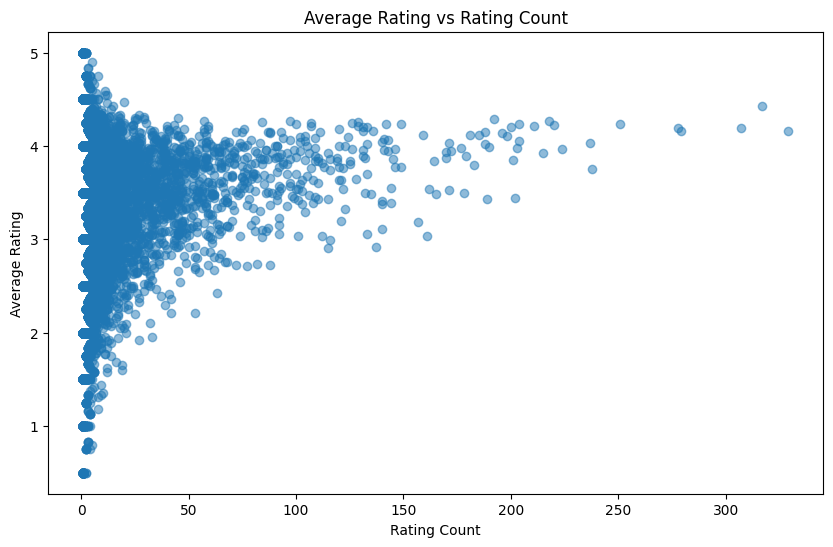
\includegraphics[width=0.5\linewidth]{average rating vs rating count.png}
    \caption{Scatterplot displaying the relationship between movie rating count and average movie rating within the MovieLens dataset.}
    \label{fig:figure1}
\end{figure}

The popularity-based recommendation system successfully identified widely enjoyed films, but it lacked personalization because recommendations were generated solely from overall rating statistics rather than individual user behavior.

\subsection{Collaborative Filtering Results}

The item-based collaborative filtering system improved personalization by producing recommendations based on user rating behavior. As mentioned in the methodology section, Pearson correlation scores were used to identify relationships between movies within the user-movie matrix. Movies with higher positive correlation values were considered more similar.

Experimental analysis showed that collaborative filtering generated more personalized recommendations than the baseline. However, as mentioned before, they often lacked genre similarity. Table 1 demonstrates this limitation using recommendations generated for ``28 Days Later (2002).'' Although several recommendations achieved strong correlation scores, many recommended films shared little genre similarity with the selected horror film, often being comedy or romance films.

These results demonstrated that collaborative filtering alone can capture statistical similarity in user rating behavior, but fails in finding similarly themed movies. Evaluating recommendation quality is often difficult because recommendation relevance depends not only on statistical similarity, but also user interpretation \cite{herlocker2004evaluating}.

\subsection{Hybrid Recommendation Results}

Experimental results showed that the hybrid recommendation model, through using collaborative filtering, combined with cosine similarity generated by the one-hot encoded genre vectors, produced recommendations with improved genre consistency and high correlation scores. Movies recommended by the hybrid system shared a strong genre overlap with the selected film compared to recommendations generated using only collaborative filtering. Cosine similarity calculations using vector-space elements helped reinforce genre relationships between movies \cite{salton1975vectorspace}.
\begin{figure}[ht]
    \centering
    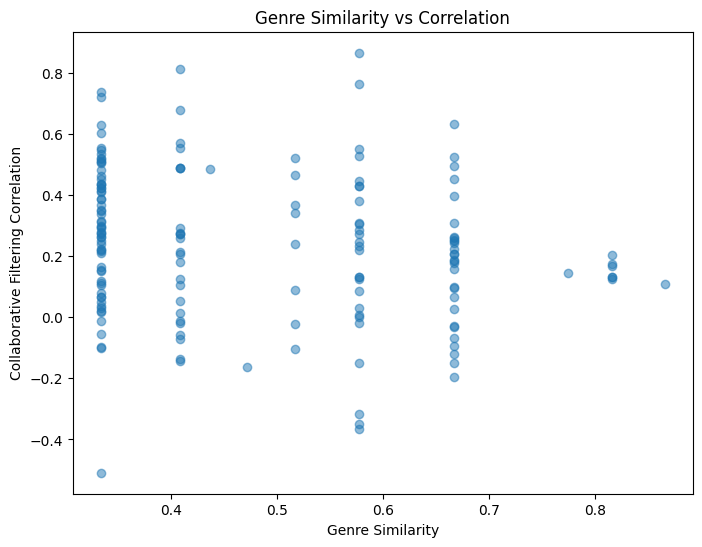
\includegraphics[width=0.5\linewidth]{genre similarity vs correlation.png}
    \caption{Scatterplot illustrating the relationship between collaborative filtering correlation scores and genre similarity scores within the hybrid recommendation model..}
    \label{fig:hybridscores}
\end{figure}
Figure \ref{fig:hybridscores} illustrates the relationship between collaborative filtering correlation scores and genre similarity score. The inclusion of genre similarity reduced the number of genre inconsistent recommendations while preserving recommendation relevance. Preserving recommendation relevance was also made a priority, giving it 70\% of the value in the hybrid score, while genre relevance was given a 30\% value. Table 2 displays the importance of both correlation scores and genre similarity for user recommendation.
\begin{table}[ht]
\centering
\small
\begin{tabular}{|p{3.8cm}|p{4.2cm}|c|c|c|}
\hline
\textbf{Recommended Movie} & \textbf{Genres} & \textbf{Correlation} & \textbf{Genre Similarity} & \textbf{Hybrid Score} \\
\hline
Star Trek II: The Wrath of Khan (1982) & Action|Adventure|Sci-Fi|Thriller & 0.865 & 0.577 & 0.779 \\
\hline
Star Trek (2009) & Action|Adventure|Sci-Fi|IMAX & 0.762 & 0.577 & 0.706 \\
\hline
In the Line of Fire (1993) & Action|Thriller & 0.811 & 0.408 & 0.690 \\
\hline
Zombieland (2009) & Action|Comedy|Horror & 0.631 & 0.667 & 0.642 \\
\hline
District 9 (2009) & Mystery|Sci-Fi|Thriller & 0.735 & 0.333 & 0.615 \\
\hline
First Knight (1995) & Action|Drama|Romance & 0.720 & 0.333 & 0.604 \\
\hline
Coneheads (1993) & Comedy|Sci-Fi & 0.678 & 0.408 & 0.597 \\
\hline
Iron Man (2008) & Action|Adventure|Sci-Fi & 0.525 & 0.667 & 0.567 \\
\hline
V for Vendetta (2006) & Action|Sci-Fi|Thriller|IMAX & 0.550 & 0.577 & 0.558 \\
\hline
Guardians of the Galaxy (2014) & Action|Adventure|Sci-Fi & 0.495 & 0.667 & 0.547 \\
\hline
\end{tabular}
\caption{Top hybrid recommendation results generated for ``28 Days Later (2002).'' By incorporating genre similarity into the recommendation process, the hybrid model produced recommendations with stronger thematic consistency while maintaining collaborative filtering relevance.}
\label{tab:hybrid_recommendations}
\end{table}


\subsection{Comparative Analysis}

Overall, the popularity-based recommendation system produced good recommendations but lacked personalization. Collaborative filtering significantly improved personalization, but often generated recommendations with inconsistent genre relationships. The hybrid recommendation system successfully balanced personalization and semantic consistency by integrating collaborative filtering with genre-based similarity calculations.

These results are consistent with prior hybrid recommendation research, which demonstrated that combining collaborative and content-based recommendation strategies can improve recommendation quality while reducing irrelevant recommendations \cite{burke2002hybrid}. The experimental results of this project demonstrate that incorporating genre-based similarity measures into collaborative filtering systems can improve consistency and personalization without significantly reducing recommendation relevance.
\section{Discussion}

The results of this project demonstrate the strengths and weaknesses of multiple recommendation system approaches. The popularity-based recommendation system provided stable and widely liked movie recommendations, but it failed to account for the preferences of individual users. While this method was effective at identifying highly rated films, it lacked the personalization necessary for modern recommendation systems used in streaming platforms. The collaborative filtering recommendation model improved personalization significantly by identifying similarities between movies based on historical user rating behavior. Recommendations generated through Pearson correlation were more tailored to user interests than those produced by the popularity-based baseline. However, experimental analysis showed that collaborative filtering alone struggled to maintain thematic consistency. Several recommendations generated for ``28 Days Later (2002)'' included comedy and romance films with no overlap in genre despite achieving high correlation scores. These findings demonstrate that statistical similarity in user ratings does not always correspond to meaningful similarity between movies. The hybrid recommendation system addressed many of these limitations by incorporating cosine similarity generated from one-hot encoded genre vectors into the recommendation process. By combining collaborative filtering similarity with genre similarity, the hybrid model was able to preserve personalization while improving recommendation consistency. Experimental results showed that the hybrid recommendation system produced recommendations with stronger genre overlap and fewer inconsistent results compared to just collaborative filtering.

\section{Limitations}

Despite these improvements, the hybrid recommendation model still contains limitations. Genre similarity alone may not fully capture thematic relationships between films. Movies that share similar genres may still differ significantly in tone, pacing, narrative structure, or target audience. Additionally, the weighting values used in the hybrid score calculation were selected experimentally and may not represent the optimal balance between collaborative filtering and genre similarity. Another limitation of this project is the reliance on user rating data from the MovieLens dataset, which is limited. Sparse rating data remains a challenge for recommendation systems, particularly for movies with limited user interaction. Furthermore, the recommendation system only utilized genre metadata and did not incorporate additional content features such as actors, directors, plot summaries, release periods, or user demographic information. Future work could improve the recommendation system by incorporating richer metadata and more advanced recommendation techniques. Additional experimentation with dynamic weighting strategies and user-specific preference modeling may also further improve recommendation quality and personalization.

\section{Code Availability}

The complete source code, preprocessing scripts, and evaluation notebooks used throughout this project are available at:

\href{https://github.com/bennywilson05/movie-recommender-project}{GitHub Repository}

\newpage
\bibliographystyle{ieeetr}
\bibliography{references}
\end{document}